% Memoria del TFG «Análisis automatizado de vídeo deportivo mediante visión por
% computador» (Padel Vision). Basada en la plantilla de la ETSII de la URJC
% (github.com/codeurjc-students/tfg-template, licencia MIT: LICENSE-plantilla).
%
% Compilar: latexmk -pdf tfg.tex   (o guardar en VS Code con LaTeX Workshop)
% Las notas \alumno{} y \tutor{} solo se ven con \drafttrue (config/config.tex).

% Clase del documento
\documentclass[12pt,twoside,titlepage,openright]{report}

% Configuración
% Preámbulo de la memoria.

%%%%%%%%%%%%%%%%%%%%%%%%%%%% Página, letra e idioma %%%%%%%%%%%%%%%%%%%%%%%%%%%%

\usepackage[a4paper,left=3cm,right=2.5cm,top=2.7cm,bottom=2.7cm,headheight=15pt]{geometry}
\usepackage[T1]{fontenc}
\usepackage{lmodern}
\usepackage[spanish,es-tabla,es-nosectiondot,es-noshorthands]{babel}
\usepackage{microtype}
\usepackage{csquotes}

% Interlineado de 1,2 sobre la letra de 11 pt (unos 16,3 pt entre líneas); párrafos sin sangría, separados por un espacio
\usepackage{setspace}
\setstretch{1.2}
\usepackage[skip=0.6\baselineskip plus 2pt,indent=0pt]{parskip}
\raggedbottom
\clubpenalty=10000
\widowpenalty=10000

% Capítulo: número grande en gris, título debajo alineado a la derecha y línea fina
\usepackage{xcolor}
\definecolor{numcap}{HTML}{B0B0B0}
\usepackage{titlesec}
\titleformat{\chapter}[display]
  {\normalfont\bfseries\raggedleft\hyphenpenalty=10000\exhyphenpenalty=10000}
  {\fontsize{90}{90}\selectfont\color{numcap}\thechapter}
  {-6pt}
  {\fontsize{32}{38}\selectfont}
  [{\vspace{4pt}\titlerule[0.8pt]}]
\titleformat{name=\chapter,numberless}[display]
  {\normalfont\bfseries\raggedleft\hyphenpenalty=10000\exhyphenpenalty=10000}
  {}
  {0pt}
  {\fontsize{32}{38}\selectfont}
  [{\vspace{4pt}\titlerule[0.8pt]}]
\titlespacing*{\chapter}{0pt}{-10pt}{36pt}
\titlespacing*{name=\chapter,numberless}{0pt}{40pt}{36pt}
\definecolor{azultitulo}{HTML}{1F2A44}
\definecolor{numcap}{HTML}{B8BCC6}
\titleformat{\chapter}[display]
  {\normalfont\bfseries\raggedleft\color{azultitulo}\hyphenpenalty=10000\exhyphenpenalty=10000}
  {\fontsize{90}{90}\selectfont\color{numcap}\thechapter}
  {-6pt}
  {\fontsize{32}{38}\selectfont}
  [{\vspace{4pt}\titlerule[0.8pt]}]
\titleformat{name=\chapter,numberless}[display]
  {\normalfont\bfseries\raggedleft\color{azultitulo}\hyphenpenalty=10000\exhyphenpenalty=10000}
  {}
  {0pt}
  {\fontsize{32}{38}\selectfont}
  [{\vspace{4pt}\titlerule[0.8pt]}]
\titleformat{\section}{\normalfont\Large\bfseries\color{azultitulo}}{\thesection}{0.8em}{}
\titleformat{\subsection}{\normalfont\large\bfseries\color{azultitulo}}{\thesubsection}{0.8em}{}

% Las listas de los índices, a interlineado sencillo (el título no cambia)
\makeatletter
\let\starttocoriginal\@starttoc
\renewcommand{\@starttoc}[1]{\begingroup\setstretch{1}\starttocoriginal{#1}\endgroup}
\makeatother

\addto\captionsspanish{%
  \renewcommand{\contentsname}{Índice}%
  \renewcommand{\appendixname}{Anexo}}

%%%%%%%%%%%%%%%%%%%%%%%%%%%% Figuras, tablas y números %%%%%%%%%%%%%%%%%%%%%%%%%%

\usepackage{graphicx}
\usepackage{xcolor}
\usepackage{amsmath,amssymb}
\usepackage{booktabs}
\usepackage{array}
\usepackage{multirow}
\usepackage{enumitem}
\usepackage{caption}
\captionsetup{font=small,labelfont=bf,skip=8pt}
\captionsetup[table]{position=top}
\usepackage{subcaption}
% [H] coloca una figura exactamente donde está en el texto, aunque deje hueco
% al final de la página: para las que se describen justo antes de aparecer
\usepackage{float}
% Ninguna figura cruza a la sección siguiente
\usepackage[section]{placeins}

% Cada figura y cada tabla dejan un pequeño margen propio por encima (14 pt), para
% que no queden pegadas al título o al texto que las precede, y su pie va junto a
% ellas: el espacio entre párrafos no se aplica dentro de figuras ni tablas.
% Figuras y tablas llevan el mismo margen: son el mismo tipo de elemento.
% El margen se añade al colocar la figura en medio del texto (en su sitio, o fija
% con [H]), no en el punto del código donde se escribe: si la figura se va a otra
% página, no deja un hueco en el texto. El \penalty0 deja cortar la página justo
% antes: sin él, una figura fija que no cabe obliga a partir por la mitad el
% párrafo que la precede.
% Las figuras pueden ocupar hasta el 90 % de lo alto de una página con texto
% debajo (por defecto, el 70 %): así dos figuras seguidas comparten página con el
% texto que las sigue, en lugar de quedar solas en una página de figuras
\renewcommand{\topfraction}{0.9}
\renewcommand{\textfraction}{0.1}
\renewcommand{\floatpagefraction}{0.8}
\setlength{\intextsep}{6pt plus 2pt minus 2pt}
\makeatletter
\patchcmd{\@addtocurcol}
  {\vskip\intextsep\box\@currbox}{\vskip\intextsep\vskip14pt\box\@currbox}
  {}{\PackageWarning{tfg}{No se pudo añadir el margen de las figuras en el texto}}
\patchcmd{\float@endH}
  {\@endfloatbox\vskip\intextsep}{\@endfloatbox\vspace*{14pt}\vskip\intextsep}
  {}{\PackageWarning{tfg}{No se pudo añadir el margen de las figuras fijas}}
\makeatother
\AtBeginEnvironment{figure}{\setlength{\parskip}{0pt}\par\penalty0}
\AtBeginEnvironment{table}{\setlength{\parskip}{0pt}\par\penalty0}

% Números según la RAE: coma decimal, espacio antes de las unidades y del %,
% y separación de miles solo a partir de cinco cifras (2377, pero 10 000)
\usepackage{siunitx}
\sisetup{
  output-decimal-marker = {,},
  group-separator = {\,},
  group-minimum-digits = 5,
}

% Diagramas (TikZ): cajas neutras y paneles de color suave por etapa. Cada
% diagrama, en figuras/
\usepackage{adjustbox} % reduce un diagrama que se pase del ancho del texto
\usepackage{tikz}
\usetikzlibrary{positioning,fit,arrows.meta,calc,backgrounds}
\definecolor{tinta}{HTML}{0b0b0b}
\definecolor{tinta2}{HTML}{52514e}
\definecolor{tenue}{HTML}{898781}
\definecolor{borde}{HTML}{b5b4aa}
\definecolor{fondo}{HTML}{f4f4f1}
\definecolor{panelaudio}{HTML}{eef3f9}
\definecolor{panelimagen}{HTML}{eef6f1}
\definecolor{panelgolpe}{HTML}{fbf4ea}
% Letra de las cajas: 9 pt fijos, el tamaño con el que se dimensionaron las cajas
% (\footnotesize crece con la letra del documento y las palabras largas se salen)
\newcommand{\letradiagrama}{\fontsize{9}{11}\selectfont}
\tikzset{
  caja/.style={draw=borde, fill=white, rounded corners=2pt, align=center,
    font=\letradiagrama, inner sep=3.5pt, minimum height=9mm, text width=21mm, text=tinta},
  entrada/.style={caja, fill=fondo},
  linea/.style={draw=tinta2, line width=0.55pt},
  flecha/.style={linea, -{Stealth[length=1.8mm]}},
  dato/.style={font=\scriptsize\itshape, text=tinta2, inner sep=1pt},
  panel/.style={rounded corners=6pt, inner sep=7pt},
  titulopanel/.style={font=\scriptsize, text=tinta2, anchor=south west, inner sep=2pt},
  seccion/.style={font=\tiny, text=tenue, anchor=north east, inner sep=1.5pt},
}
% Segunda línea, más pequeña y gris, dentro de una caja
\newcommand{\subcaja}[1]{\\[-1pt]{\scriptsize\color{tenue}#1}}
% Iconos de los diagramas: el jugador, un pictograma de remate como los de la
% figura de la ventana (0,66 de alto, pies en el origen), y la pelota de pádel
% (radio 0,085, centrada). El color se pasa al usarlos: {jugador=tinta}.
\definecolor{pelota}{HTML}{e2e23c}
\tikzset{
  pics/jugador/.style={code={
    \fill[#1] (0.015,0.44) circle (0.052);
    \draw[#1, line width=1.6pt, line cap=round] (0,0.35) -- (0,0.19);
    \draw[#1, line width=1.1pt, line cap=round, line join=round]
      (0,0.19) -- (-0.075,0.0) (0,0.19) -- (0.075,0.0)
      (0,0.33) -- (0.065,0.43) -- (0.085,0.52)
      (0,0.33) -- (-0.07,0.39) -- (-0.085,0.47);
    \draw[#1, line width=0.8pt, line cap=round] (0.085,0.52) -- (0.095,0.56);
    \fill[#1] (0.105,0.615) ellipse [x radius=0.032, y radius=0.045];
  }},
  pics/pelota/.style={code={
    \fill[#1, draw=tinta, line width=0.45pt] (0,0) circle (0.085);
    \draw[white, line width=0.55pt]
      (-0.07,0.035) .. controls (-0.02,-0.025) and (0.02,-0.025) .. (0.07,0.035);
  }},
}

%%%%%%%%%%%%%%%%%%%%%%%%%%%% Órdenes de terminal %%%%%%%%%%%%%%%%%%%%%%%%%%%%%%%%%

% Bloques con las órdenes que se escriben en la terminal: letra monoespaciada
% sobre el fondo gris de los diagramas, el «$» del indicador en gris y los
% comentarios en gris y cursiva. Uso: \begin{lstlisting}[style=terminal] ...
% \end{lstlisting} (el editor lo reconoce como código; con \begin{terminal} sale
% igual en el PDF, pero el editor colorea los «$» como si abrieran fórmulas)
\usepackage{listings}
\lstdefinestyle{terminal}{
  language=bash,
  basicstyle=\ttfamily\small\color{tinta},
  keywordstyle=\color{tinta},
  commentstyle=\color{tenue}\itshape,
  backgroundcolor=\color{fondo},
  frame=single, rulecolor=\color{borde}, framerule=0.4pt, framesep=5pt,
  xleftmargin=6pt, xrightmargin=6pt,
  aboveskip=10pt, belowskip=8pt,
  columns=fullflexible, keepspaces=true, showstringspaces=false,
  breaklines=true,
  literate={\$}{{\textcolor{tenue}{\$}}}1
           {á}{{\'a}}1 {é}{{\'e}}1 {í}{{\'i}}1 {ó}{{\'o}}1 {ú}{{\'u}}1 {ñ}{{\~n}}1,
}
\lstnewenvironment{terminal}{\lstset{style=terminal}}{}

%%%%%%%%%%%%%%%%%%%%%%%%%%%% Bibliografía %%%%%%%%%%%%%%%%%%%%%%%%%%%%%%%%%%%%%%%%

% Estilo IEEE (numérico, con las citas seguidas agrupadas: [1]-[4]) y los textos
% de la bibliografía en español
\usepackage[style=ieee,citestyle=ieee-comp,backend=biber]{biblatex}
\addbibresource{bibliografia.bib}
\renewcommand*{\bibfont}{\small}
\stdpunctuation % la coma tras las comillas, como en español («…», y no «…,»)
\DefineBibliographyStrings{spanish}{
  artno   = {art\adddot\addnbspace n\sptext{o}},
  jourser = {col\adddot},
  url     = {[En línea]\adddot\addspace Disponible en},
  urlseen = {Consultado el},
}

%%%%%%%%%%%%%%%%%%%%%%%%%%%% Siglas y acrónimos %%%%%%%%%%%%%%%%%%%%%%%%%%%%%%%%%%

% La primera vez que se usa una sigla se escribe completa; después, solo la sigla
\usepackage{acro}
\acsetup{
  make-links = true,
  list/name = {Siglas y acrónimos},
  list/heading = capitulo-en-indice,
}
\NewAcroTemplate[heading]{capitulo-en-indice}{%
  \chapter*{\acrolistname}%
  \addcontentsline{toc}{chapter}{\acrolistname}%
  \markboth{\MakeUppercase{\acrolistname}}{\MakeUppercase{\acrolistname}}}
% Siglas y acrónimos de la memoria (paquete acro). En el texto se usa \ac{clave}.
% El desarrollo corresponde letra a letra con la sigla: si es inglesa, en inglés
% y en cursiva; si es española, en español (README.md, «Cómo se escribe»).
% Formato de cada entrada:
%   \DeclareAcronym{crnn}{
%     short = CRNN,
%     long  = \textit{convolutional recurrent neural network},
%   }

\DeclareAcronym{bst}{
  short = BST,
  long  = \textit{Badminton Stroke-type Transformer},
}
\DeclareAcronym{crnn}{
  short = CRNN,
  long  = \textit{convolutional recurrent neural network},
}
\DeclareAcronym{fft}{
  short = FFT,
  long  = \textit{fast Fourier transform},
}
\DeclareAcronym{gru}{
  short = GRU,
  long  = \textit{gated recurrent unit},
}


%%%%%%%%%%%%%%%%%%%%%%%%%%%% Cabeceras y pies de página %%%%%%%%%%%%%%%%%%%%%%%%%%

\usepackage{fancyhdr}
\renewcommand{\chaptermark}[1]{\markboth{\chaptername\ \thechapter.\ #1}{}}
\renewcommand{\sectionmark}[1]{\markright{\thesection\ #1}}
\fancypagestyle{fancy}{%
  \fancyhf{}%
  \fancyhead[L]{\small\itshape\leftmark}%
  \fancyhead[R]{\small\rightmark}%
  \fancyfoot[C]{\small\thepage}%
  \renewcommand{\headrulewidth}{0.4pt}%
  \renewcommand{\footrulewidth}{0pt}}
\fancypagestyle{plain}{%
  \fancyhf{}%
  \fancyfoot[C]{\small\thepage}%
  \renewcommand{\headrulewidth}{0pt}%
  \renewcommand{\footrulewidth}{0pt}}

%%%%%%%%%%%%%%%%%%%%%%%%%%%% Datos fijos %%%%%%%%%%%%%%%%%%%%%%%%%%%%%%%%%%%%%%%%%

\newcommand{\escuela}{Escuela Técnica Superior\\de Ingeniería Informática}
\newcommand{\escuelalargo}{Escuela Técnica Superior de Ingeniería Informática}
\newcommand{\universidad}{Universidad Rey Juan Carlos}
\newcommand{\logoUniversidad}{config/logos/logoURJC.pdf}

%%%%%%%%%%%%%%%%%%%%%%%%%%%% Comentarios de revisión %%%%%%%%%%%%%%%%%%%%%%%%%%%%%

% \tutor{}, \cotutor{} y \alumno{} solo se ven con \drafttrue
\newif\ifdraft
\drafttrue
% Comentarios de revisión: se ven en el borrador (\drafttrue) y desaparecen en
% la versión final (\draftfalse)
\ifdraft
  \usepackage{todonotes}
\else
  \usepackage[disable]{todonotes}
\fi

\newcommand{\tutor}[1]{\todo[color=red!40, inline]{\footnotesize \textbf{Tutor:} #1}}
\newcommand{\cotutor}[1]{\todo[color=green!40, inline]{\footnotesize \textbf{Cotutor:} #1}}
\newcommand{\alumno}[1]{\todo[color=blue!40, inline]{\footnotesize \textbf{Alumno:} #1}}


%%%%%%%%%%%%%%%%%%%%%%%%%%%% Enlaces y referencias cruzadas %%%%%%%%%%%%%%%%%%%%%%%

% Enlaces sin color, para que la versión impresa salga en negro
\usepackage{hyperref}
\hypersetup{
  hidelinks,
  bookmarksnumbered,
  pdftitle  = {\titulotrabajo},
  pdfauthor = {\nombreautor},
  pdflang   = {es-ES},
}

% \cref{fig:x} escribe «figura 2.4» con el enlace; \Cref, a principio de frase
\usepackage[spanish]{cleveref}
\crefname{table}{tabla}{tablas}
\Crefname{table}{Tabla}{Tablas}
\crefname{appendix}{anexo}{anexos}
\Crefname{appendix}{Anexo}{Anexos}
\crefname{section}{sección}{secciones}
\Crefname{section}{Sección}{Secciones}
\crefname{subsection}{sección}{secciones}
\Crefname{subsection}{Sección}{Secciones}

\usepackage{emptypage} % sin cabeceras en las páginas en blanco antes de cada capítulo

% Datos del trabajo (tal como figuran en la plataforma de TFG)
\newcommand{\nombreautor}{Jorge Sánchez Aguilar}
\newcommand{\nombretutor}{Isaac Martín de Diego}
\newcommand{\nombrecotutor}{Víctor Aceña Gil}
\newcommand{\titulotrabajo}{Análisis automatizado de vídeo deportivo mediante visión por computador}
\newcommand{\grado}{Grado en Ingeniería Informática}
\newcommand{\curso}{2026/2027}

%%%%%%%%%%%%%%%%%%%%%%%%%%%%%%%%%%%%%%%%%%%%%%%%%%%%%%%%%%%%%%%%%%%%%%%
%                           Inicio del documento
%%%%%%%%%%%%%%%%%%%%%%%%%%%%%%%%%%%%%%%%%%%%%%%%%%%%%%%%%%%%%%%%%%%%%%%

\begin{document}

\pagestyle{plain}

%%%%%%%%%%%%%%%%%%%%%%%%%%%%%%%%%%%% Portada %%%%%%%%%%%%%%%%%%%%%%%%%%%%%%%%%%

% Portada según el modelo del Anexo I del Reglamento Específico del TFG de la
% ETSII (Junta de Escuela, 16 de enero de 2026).

\begin{titlepage}
\selectlanguage{spanish}

% Logo
\begin{center}
    \includegraphics[scale=0.7]{\logoUniversidad}
\end{center}

\vspace{1.5cm}

% Escuela, grado y curso
\begin{center}
    % One line, as in the official model: centred, allowed into the margins
    \makebox[0pt][c]{\textbf{\MakeUppercase{\escuela}}}

    \vspace{1cm}

    \textbf{\MakeUppercase{\grado}}

    \vspace{0.4cm}

    \textbf{Curso Académico \curso}

    \vspace{1.2cm}

    \textbf{Trabajo de Fin de Grado}
\end{center}

\vspace{1.8cm}

% Título
\begin{center}
    \begin{large}
        \textbf{\MakeUppercase{\titulotrabajo}}
    \end{large}
\end{center}

\vfill

% Autor y tutores
\begin{center}
    \begin{tabular}{@{}l@{\hspace{1.5em}}l@{}}
        \textbf{Autor:}   & \nombreautor \\[1.2em]
        \textbf{Tutores:} & \nombretutor \\
                          & \nombrecotutor \\
    \end{tabular}
\end{center}

\vspace{2cm}

\end{titlepage}

\hypersetup{pageanchor=true}

\normalsize
\afterpage{\blankpage} % Página en blanco para que las secciones siguientes empiecen en página impar


% Estilo de párrafo de los preliminares
\setlength{\parskip}{0.75em}
\renewcommand{\baselinestretch}{1.25}
\spacing{1}

\pagenumbering{Roman}
\setcounter{page}{2}

%%%%%%%%%%%%%%%%%%%%%%%%% Licencia %%%%%%%%%%%%%%%%%%%%%%%%%%%

% Licencia de la memoria, en el reverso de la portada (art. 8 y anexo IV del
% reglamento). Detalles en https://ofilibre.urjc.es/guias/tfg-abierto/
\thispagestyle{empty}
\vspace*{\fill}

\begin{flushright}

\includegraphics[scale=0.6]{config/cc/by-sa.eps}

\noindent © 2026 \nombreautor \\
Algunos derechos reservados \\
Este documento se distribuye bajo la licencia \\
«Atribución-CompartirIgual 4.0 Internacional» de Creative Commons, \\
disponible en \\
\url{https://creativecommons.org/licenses/by-sa/4.0/deed.es}
\end{flushright}


%%%%%%%%%%%%%%%%%%%%%%%%% Agradecimientos %%%%%%%%%%%%%%%%%%%%%%%%%%%

\chapter*{Agradecimientos}

\alumno{Opcional. Breves agradecimientos o dedicatoria.}

\afterpage{\blankpage}

%%%%%%%%%%%%%%%%%%%%%%%%%%%%%%%%%%%% Resumen %%%%%%%%%%%%%%%%%%%%%%%%%%%%%%%%%%

\chapter*{Resumen}

% !TEX root = ../tfg.tex

\noindent\textbf{Palabras clave:}


\afterpage{\blankpage}

%%%%%%%%%%%%%%%%%%%%%%%%%%%%%%%%%%%% Abstract %%%%%%%%%%%%%%%%%%%%%%%%%%%%%%%%%

\chapter*{Abstract}

% !TEX root = ../tfg.tex

\alumno{Traducción del resumen al inglés. Opcional según la normativa; útil si el trabajo da lugar a una publicación.}

\mbox{} \bigskip

\noindent \textbf{Keywords}: \alumno{Las mismas que en el resumen, en inglés.}


\afterpage{\blankpage}

%%%%%%%%%%%%%%%%%%%%%%%%%%%%%%%%%%%% Índices %%%%%%%%%%%%%%%%%%%%%%%%%%%%%%%%%%

\setlength{\parskip}{1pt}
\renewcommand{\baselinestretch}{1}
\renewcommand{\contentsname}{Índice de contenidos}

\dominitoc
\setcounter{minitocdepth}{2}
\setlength{\mtcindent}{0pt}

\tableofcontents
\afterpage{\blankpage}

\listoffigures
\afterpage{\blankpage}
\addcontentsline{toc}{chapter}{\listfigurename}
\adjustmtc

\listoftables
\afterpage{\blankpage}
\addcontentsline{toc}{chapter}{\listtablename}
\adjustmtc

%%%%%%%%%%%%%%%%%%%%%%% Cabeceras y pies de página %%%%%%%%%%%%%%%%%%%%%%%

\setlength{\headheight}{15pt}
\renewcommand{\chaptermark}[1]{\markboth{Capítulo \thechapter.\ #1}{}}
\pagestyle{fancy}
\fancyhf{}
\fancyhead[LO]{\leftmark}
\fancyhead[RO]{}
\fancyhead[RE]{\nouppercase\rightmark}
\fancyhead[LE]{}
\fancyfoot[C]{\thepage}

%%%%%%%%%%%%%%%%%%%%%%%%%%%%%% Capítulos %%%%%%%%%%%%%%%%%%%%%%%%%%%%%%%%%%%%
% La extensión (40-60 páginas) se cuenta desde la introducción y sin anexos
% (art. 16 del reglamento de la ETSII).

\setlength{\parskip}{0.75em}
\renewcommand{\baselinestretch}{1.25}
\spacing{1}
\cleardoublepage
\pagenumbering{arabic}
\setcounter{page}{1}

\chapter{Introducción}
\label{cap:introduccion}
% !TEX root = ../tfg.tex

\section{Motivación y antecedentes}
\label{sec:motivacion}

% IDEAS (borrar antes de pasar la memoria al tutor)
% - El problema: analizar el pádel; el paso siguiente, que nadie ha dado, es
%   clasificar el tipo de golpe.
% - El hueco, dicho con precisión («hasta donde se ha podido comprobar»): no hay
%   trabajos publicados ni herramientas abiertas que clasifiquen el tipo de golpe
%   a partir del vídeo. Matices: Cartes Domínguez (2023) lo clasifica con una
%   pulsera de sensores, no con vídeo; hay aplicaciones comerciales (aiball,
%   Padelytics, Padel AI) que no publican ni su método ni su precisión. El
%   estado del arte lo respalda.

\section{Objetivos generales y específicos}
\label{sec:objetivos}

% IDEAS (borrar antes de pasar la memoria al tutor)
% - En prosa y con conectores, no en lista («En primer lugar se quiso…»).
% - Para quién: clubes que quieran este análisis y tengan, o pongan, una cámara
%   fija al fondo de la pista, en alto.
% - General: que esos clubes tengan una herramienta de análisis de nivel
%   profesional para mejorar.
% - Listón: que funcione lo bastante bien para usarse de verdad, no una cifra
%   fijada de antemano.
% - Específicos: detectar el instante de cada golpe; identificar al jugador;
%   clasificar el tipo (derecha, revés, remate, saque); el visor (estadísticas
%   por jugador: golpes por tipo, total, mapa de calor; saltar al instante de
%   cada golpe; que sea útil).
% - El tipo no va solo: sin cuándo y quién no hay estadísticas por jugador.
%   Cadena; la pieza nueva es la última.
% - Decorte et al., base del cuándo y el quién: no reinventar un método que
%   funcionaba; compararse solo para comprobar la reimplementación.
% - No son objetivos: los datos etiquetados (medio: no existían con el tipo; se
%   cuentan en Datos); la evaluación por torneos (va en Experimentos).
% - Alcance, al final y en pocas frases: fuera el marcador y el resultado;
%   bandeja, víbora y dejada; cámaras móviles o a ras de pista; partidos
%   completos (trabaja por puntos); saber quién es cada jugador entre puntos.
%   Evaluado con retransmisiones (las grabaciones anotadas de que se dispone,
%   cumplen la condición de cámara); otras alturas = trabajo futuro (PADELVIC,
%   cuatro alturas).
% - Para Descripción informática o Datos (no para aquí): entra el punto ya
%   cortado, con audio y sin anotar, y la pista se marca a mano una vez por
%   cámara (cuatro esquinas y extremos de la red); sale, por cada golpe,
%   instante, jugador y tipo; todo golpe recibe uno de los cuatro tipos (sin
%   «sin clasificar»; un 7 % de los etiquetados no es ninguno); los tipos se
%   agrupan por gesto (volea de derecha = derecha); J1-J4 son posiciones dentro
%   del punto (J1-J2 al fondo), no personas. Posible: por qué es difícil.
% - Figura: figuras/problema.pdf (scripts/build_problem_figure.py). VIGO_14
%   (Danish Padel Open), revés de J3 a 4,52 s, con los modelos entregados, que
%   vieron este punto al entrenar: ilustra la salida, no demuestra el acierto;
%   los modelos entrenados sin VIGO también aciertan este golpe. Pie: solo el
%   torneo (CVSPORTS se cita en Datos). Se puede mover a donde encaje mejor.

\begin{figure}[htbp]
  \centering
  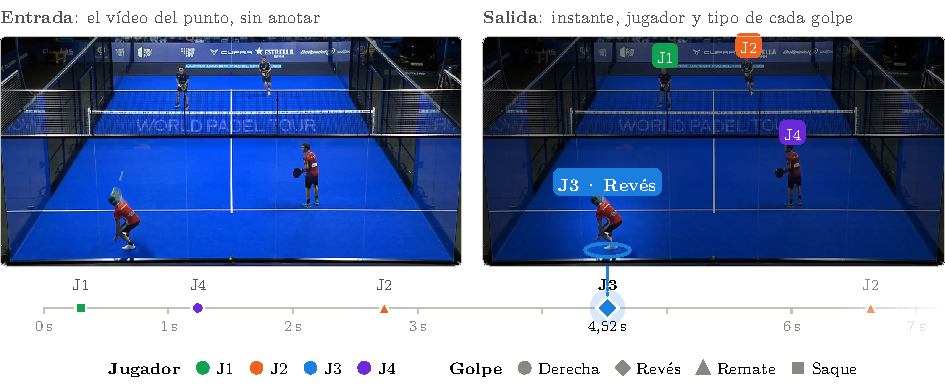
\includegraphics{figuras/problema}
  \caption{Un punto antes y después de procesarlo (Danish Padel Open 2023).}
  \label{fig:problema}
\end{figure}

\section{Metodología del trabajo}
\label{sec:metodologia}


\chapter{Objetivos}
\label{cap:objetivos}
% !TEX root = ../tfg.tex

% IDEAS (borrar antes de pasar la memoria al tutor)
% - Para quién: clubes que quieran este análisis y tengan, o pongan, una cámara
%   fija al fondo de la pista, en alto.
% - Entra: el vídeo crudo de un punto, con audio, sin ninguna anotación. Única
%   preparación: marcar la pista a mano una vez por cámara.
% - Sale: por cada golpe, instante, jugador y tipo (derecha, revés, remate,
%   saque; agrupados por gesto: una volea de derecha es derecha).
% - El tipo no va solo: sin cuándo y quién no hay estadísticas por jugador.
%   Cadena; la pieza nueva es la última.
% - Listón: que funcione lo bastante bien para usarse de verdad, no una cifra
%   fijada de antemano.
% - Decorte et al., base del cuándo y el quién: no reinventar un método que
%   funcionaba; compararse solo para comprobar la reimplementación.
% - Visor: estadísticas de juego por jugador (golpes por tipo, total, mapa de
%   calor) y saltar al instante de cada golpe. Que sea útil.
% - Objetivos: detectar el instante; identificar al jugador; clasificar el tipo;
%   el visor.
% - No son objetivos: los datos etiquetados (medio: no existían; una línea en el
%   problema, el resto en Datos); la evaluación por torneos (metodología).
% - Fuera: marcador y resultado; bandeja, víbora, dejada; cámaras móviles o a ras
%   de pista; partidos completos (trabaja por puntos). Evaluado con
%   retransmisiones (únicas grabaciones anotadas, cumplen la condición de
%   cámara); otras alturas = trabajo futuro (PADELVIC, cuatro alturas).
% - Figura en el problema, de ejemplo y sin flechas: (a) fotograma crudo de un
%   punto; (b) lo que sale: línea de tiempo con todos los golpes y, sobre el
%   mismo fotograma, quién da el golpe de ese instante y de qué tipo. Punto de
%   VIGO, salida de los modelos entrenados sin ese torneo (chain_cv), golpe
%   correcto en instante, jugador y tipo.
% - Citas: Decorte et al.; CVSPORTS en el pie de la figura.

\section{Descripción del problema}
\label{sec:problema}

\section{Objetivo general}
\label{sec:objetivo-general}

\section{Objetivos específicos}
\label{sec:objetivos-especificos}

\section{Alcance}
\label{sec:alcance}


\chapter{Estado del arte y estudio de alternativas}
\label{cap:estado-del-arte}
% !TEX root = ../tfg.tex

\alumno{Extensión prevista: unas 8 páginas. Fuente: docs/bibliography.md y docs/research-shot-detection-2026.md.}

\section{Análisis automático en deportes de raqueta}
\alumno{Trabajos previos y datasets de pádel (Novillo et al., Decorte et al., PadelTracker100, CVSPORTS).}

\section{Detección del instante del golpe}
\alumno{Por imagen frente a por audio.}

\section{Detección de personas, seguimiento y pelota}
\alumno{YOLO, ByteTrack, TrackNet.}

\section{Reconocimiento de acciones a partir del esqueleto}
\alumno{ST-GCN, PoseConv3D, TemPose, BST.}

\section{Alternativas estudiadas y descartadas}
\alumno{Cada una con su medida: pose y pelota frente a audio para detectar el golpe, pista automática frente a manual, ST-GCN y PoseConv3D frente a BST. Fuente: ADR y docs/experiments.md.}


\chapter{Metodología}
\label{cap:metodologia}
% !TEX root = ../tfg.tex

\alumno{Extensión prevista: unas 4 páginas.}

\section{Metodología de desarrollo}
\alumno{Desarrollo incremental por niveles, decisiones registradas (ADR) y bitácora de experimentos.}

\section{Metodología experimental}
\alumno{Validación dejando torneos enteros fuera, medida con la configuración exacta del sistema, intervalos de confianza y evidencias regenerables con un script.}

\section{Herramientas y entorno}
\alumno{Incluye una frase que remita al anexo de uso de herramientas de IA.}

\section{Planificación}
\alumno{De julio a diciembre de 2026.}


\chapter{Descripción informática}
\label{cap:descripcion-informatica}
% !TEX root = ../tfg.tex

Los puntos que se van a tratar durante este capítulo.
A lo largo de esta sección se detallará la arquitectura definida para identificar cada golpe. Para ello, el sistema utiliza información de audio e imágenes.
A lo largo de esta sección se detallará la arquitectura definida para identificar cada golpe. Para ello, el sistema utiliza información de audio e imágenes.

\section{Arquitectura}
\label{sec:arquitectura}

A lo largo de esta sección se detallará la arquitectura definida para identificar cada golpe.
Para ello, el sistema utiliza información de audio e imágenes.

Como paso previo al tratamiento de vídeo será necesario marcar manualmente las seis referencias espaciales que delimitan el contorno de la pista, así como la ubicación de la red.
Estas anotaciones se podrán reutilizar siempre y cuando no varíe la ubicación y orientación de la cámara.
Se probó otra alternativa de detección automática pero los resultados no eran suficientemente fiables.

El proceso arranca con un punto de pádel grabado desde una cámara fija.
Esta deberá estar situada al fondo de la pista y con una cierta elevación sobre la misma.

Utilizando los vértices previamente anotados, el sistema es capaz de localizar a los jugadores en la pista, descartando por tanto al resto de personas.
A continuación, atribuye cada golpe a un jugador y clasifica el mismo.
Como paso final, devuelve como salida el vídeo procesado y el conjunto de datos.
Todo este flujo de información queda reflejado en la \cref{fig:flujo}.

\begin{figure}[htbp]
  \centering
  % Flujo de procesamiento de un punto (sección «Arquitectura»), con el audio arriba y la imagen debajo.
% Colores y estilos en config/config.tex. Las tres entradas llegan por separado
% a «¿Quién?»; el voto pasa al clasificador la identidad del golpeador, cuya pose y
% pelota clasifica, como hace resolve_shots en padel_ml.rally_analysis. Subtítulo
% en una caja solo si añade algo: el modelo o el método.
\begin{adjustbox}{max width=\linewidth}
\begin{tikzpicture}
  % Entrada, centrada entre las dos ramas
  \node[entrada, text width=15mm] (P) at (-0.5,2.125) {Punto grabado\subcaja{vídeo y audio}};
  % Audio
  \node[caja] (A1) at (2.65,3.9) {Espectrograma\subcaja{log-Mel}};
  \node[caja] (A2) at (5.2,3.9) {Red CRNN};
  % Imagen
  \node[caja] (J1) at (2.65,1.075) {Personas y pose\subcaja{YOLO26-pose}};
  \node[caja] (J2) at (5.2,1.075) {Jugadores};
  \node[caja] (J3) at (7.75,1.075) {Identidad\subcaja{J1--J4}};
  \node[caja] (B1) at (2.65,-0.375) {Pelota\subcaja{TrackNet}};
  \node[caja] (B2) at (5.2,-0.375) {Trayectoria};
  % Por cada golpe
  \node[caja, text width=21mm] (Q) at (11.45,3.150) {¿Quién?\subcaja{voto por cercanía}};
  \node[aporta, text width=21mm] (T) at (11.45,1.100) {¿Qué golpe?\subcaja{BST}};
  % Salida: lo que lee el visor (vídeo procesado y datos del punto)
  \node[caja, text width=24mm] (R) at (14.7,2.625) {Vídeo procesado y datos de cada golpe};
  \node[caja, text width=24mm] (W) at (14.7,1.145) {Visor web};

  \begin{scope}[on background layer]
    \node[panel, fill=panelaudio, fit=(A1)(A2)] (gA) {};
    \node[panel, fill=panelimagen, fit=(J1)(J2)(J3)(B1)(B2)] (gI) {};
    \node[panel, fill=panelgolpe, fit=(Q)(T)] (gG) {};
  \end{scope}
  \node[titulopanel] at (gA.north west) {AUDIO \textperiodcentered{} cuándo};
  \node[titulopanel] at (gI.north west) {IMAGEN \textperiodcentered{} fotograma a fotograma};
  \node[titulopanel] at (gG.north west) {POR CADA GOLPE};

  % Del punto a las dos ramas: una flecha a cada una
  \draw[flecha] (P.east) -- ++(2.5mm,0) |- (gA.west);
  \draw[flecha] (P.east) -- ++(2.5mm,0) |- (gI.west);
  \draw[flecha] (A1) -- (A2);
  \draw[flecha] (J1) -- (J2);
  \draw[flecha] (J2) -- (J3);
  \draw[flecha] (B1) -- (B2);
  % Las tres entradas llegan por separado a «¿Quién?»
  \coordinate (xA2) at ($(gG.west)+(-6mm,0)$);
  \coordinate (xJ3) at ($(gG.west)+(-3.5mm,0)$);
  \coordinate (xB2) at ($(gG.west)+(-1mm,0)$);
  \draw[flecha] (A2.east) -- (A2.east -| xA2) node[dato, pos=0.5, above] {instantes}
    |- ($(Q.west)+(0,2.7mm)$);
  \draw[flecha] (J3.east) -- (J3.east -| xJ3) |- (Q.west);
  \draw[flecha] (B2.east) -- (B2.east -| xB2)
    |- ($(Q.west)+(0,-2.7mm)$);
  % El voto pasa la identidad del golpeador al clasificador, y de este sale el golpe completo
  \draw[flecha] (Q) -- (T) node[dato, midway, left] {identidad};
  \draw[flecha] (T.east) -- ++(3mm,0) |- (R.west);
  \draw[flecha] (R) -- (W);
\end{tikzpicture}
\end{adjustbox}

  \caption{Flujo de procesamiento de un punto.}
  \label{fig:flujo}
\end{figure}

Como se observa en la figura, el procesamiento se divide en dos ramas independientes, una para el audio y otra para la imagen.
La rama de audio~\cite{decorte2024padel} utiliza el sonido para detectar el instante en el que se produce el golpe (\cref{sec:instante}).
Por otro lado, la rama de imagen se encarga de dos funciones principales, por un lado asigna un identificador a cada jugador (\cref{sec:jugadores}), y por otro lado detecta la pelota (\cref{sec:pelota}).

Para cada golpe detectado por la rama de audio se recoge un determinado número de fotogramas previos y posteriores a la detección.
Dichos fotogramas permiten clasificar el golpe y el jugador que lo ha realizado.

Como se indicaba anteriormente, se obtienen el vídeo procesado y lo que es más importante aún, el conjunto de datos que permiten el análisis del punto y su visualización en el visor web.

\section{Componentes del sistema}
\label{sec:componentes}

A lo largo de esta sección se detallará la arquitectura definida para identificar cada golpe.
Para ello, el sistema utiliza información de audio e imágenes.
Me parece bien, con un matiz de redacción: no digas que todos se eligieron por prueba y error, porque algunos sí están medidos (los 1920 px, la ventana de ±4). Algo como: «los valores que no se justifican explícitamente, como umbrales o tamaños de ventana menores, se fijaron de forma empírica». Así no hay que justificarlos uno a uno, y lo medido sigue siendo medido. AAAAAAAAAAAAAAAAAAAAAAAAAAAAAAAAAAAAAAAAAAAAAAAAAAAAAAAAAAAAAAAAAAAAAAAAAAAAAAAAAAAAAAA

\subsection{Instante del golpe}
\label{sec:instante}

Aunque el enfoque inicial del proyecto consistía en identificar el instante en el que un jugador golpea la pelota basándose exclusivamente en el análisis visual de las imágenes, finalmente fue descartado dada la dificultad que entraña detectar y hacer seguimiento de la trayectoria de la pelota.
Y esta dificultad viene dada por varios motivos, el tamaño de la pelota, la alta velocidad a la que se mueve y el hecho de que la pelota no permanece siempre visible.
Se probó una alternativa basada en la imagen, a partir de la pose de los jugadores y la posición de la pelota, pero detectaba menos golpes y con más errores (\cref{tab:deteccion}).

\begin{table}[htbp]
  \centering
  \caption{...}
  \label{tab:deteccion}
  \begin{tabular}{lccc}
\toprule
\textbf{Entrada} & \textbf{Precisión} & \textbf{\textit{Recall}} & \textbf{F1} \\
\midrule
Imagen (postura y pelota) & \num{0.792} & \num{0.851} & \num{0.821} \\
Audio & \num{0.946} & \num{0.936} & \num{0.941} \\
\bottomrule
\end{tabular}

\end{table}

Es por ello por lo que se decidió utilizar otro método basado en el reconocimiento de un golpe por el sonido~\cite{decorte2024padel} que es emitido cuando un jugador golpea la pelota.

Un golpe en pádel tiene un sonido característico que el micrófono capta. Esto permite saber en qué momento exacto hay un golpe para poder analizar los fotogramas que rodean al golpe en el siguiente paso del flujo.
El sonido se analiza con un espectrograma (representación visual del cambio de frecuencia de una señal de audio a lo largo del tiempo) donde los golpes suelen ser representados por rayas verticales, aunque no todos ellos se muestran de la misma manera (un golpe cortado suena distinto a un remate).
También es importante tener en consideración que existe ruido de fondo, como gritos del público o de los jugadores.
Esto implica que no se puede asumir que todo pico en el espectrograma es un golpe.
La \cref{fig:espectrogramas} muestra cómo se ve el espectrograma en dos momentos distintos de un punto.

\begin{figure}[htbp]
  \centering
  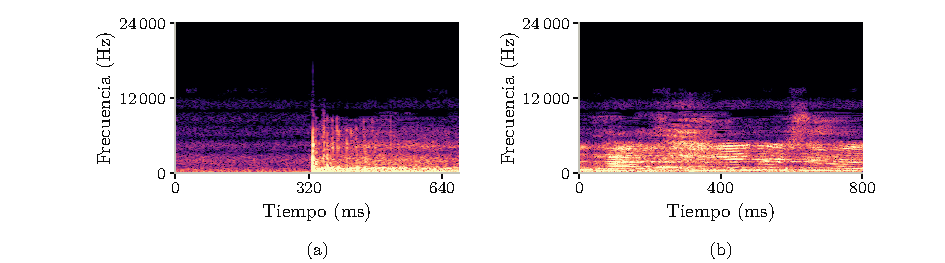
\includegraphics{figuras/espectrogramas}
  \caption{Espectrograma de un remate (a). Espectrograma de un tramo sin golpe (b).}
  \label{fig:espectrogramas}
\end{figure}

Para poder distinguir entre golpe y ruido de fondo se necesita entrenar un modelo predictivo que aprenda a diferenciar entre ambos.
Para ello se utiliza un \textit{dataset} previamente anotado~\cite{decorte2024padel} con el inicio y fin del sonido del impacto.
En total se dispone de 2377 golpes etiquetados distribuidos a lo largo de 99 puntos en distintos torneos.

La entrada del modelo es un espectrograma \textit{log-Mel}, que agrupa las frecuencias similar a la interpretación del sonido que hace el oído humano, de 40 bandas en un rango de 0--24~kHz calculado con un solape de un 50\% y una ventana \acs{fft} (\acl{fft}) de tamaño 2048, dividido en secuencias de 256 \textit{frames}.
Es importante mencionar que no se dispone de rangos infrasonido y ultrasonido porque los vídeos del \textit{dataset} están comprimidos y el algoritmo de compresión los descartó.

La arquitectura base del modelo utilizado para detectar golpes a partir de su sonido se basa en una adaptación del modelo SED-net~\cite{adavanne2017sed} con dos capas \acs{gru} (\acl{gru}) bidireccionales.
La red neuronal final tiene un total de 114 561 parámetros y las capas adaptadas se muestran en la \cref{tab:red-audio}. La red neuronal se entrenó con un optimizador AdamW~\cite{loshchilov2019adamw}, con una tasa de aprendizaje de 0,001 y con \textit{batches} de 32 secuencias.

\begin{table}[htbp]
  \centering
  \caption{Capas de la red de detección de golpes.}
  \label{tab:red-audio}
  \begin{tabular}{lcc}
\toprule
\textbf{Tipo de capa} & \textbf{Hiperparámetros} & \textbf{Activación} \\
\midrule
conv2D & $1 \to 64$, $3 \times 3$, $1 \times 1$ & ReLU \\
maxpool & $5 \times 1$ & - \\
conv2D & $64 \to 64$, $3 \times 3$, $1 \times 1$ & ReLU \\
maxpool & $2 \times 1$ & - \\
conv2D & $64 \to 64$, $3 \times 3$, $1 \times 1$ & ReLU \\
maxpool & $2 \times 1$ & - \\
reorganización & $64 \times 2 \times 256 \to 256 \times 128$ & - \\
GRU bidireccional & $256 \times 128 \to 256 \times 64$ & tanh \\
GRU bidireccional & $256 \times 64 \to 256 \times 32$ & tanh \\
densa en el tiempo & $256 \times 32 \to 256 \times 32$ & ReLU \\
densa en el tiempo & $256 \times 32 \to 256 \times 1$ & sigmoide \\
\bottomrule
\end{tabular}

\end{table}

La salida de dicha red es la probabilidad entre 0 y 1 de que haya un golpe en cada instante.
Cada máximo local de esa curva que supere 0,5 se considera un golpe, y como un mismo golpe podría dar dos máximos casi seguidos se descartan los que están a menos de 170~ms del anterior.

\subsection{Jugadores}
\label{sec:jugadores}

Los vídeos de grabaciones de pádel con los que se ha trabajado tienen la cámara situada en un extremo de la pista.
Es por ello que la imagen estará siempre en perspectiva y por tanto distorsionada.
Esto se traduce en que una misma distancia en píxeles equivale a diferentes longitudes reales en función del lugar de la pista en que se encuentre.

Esta distorsión se resuelve utilizando puntos de referencia conocidos, como los vértices de la pista de tamaño estándar $10 \times 20$~m, con los que se calcula una matriz de $3 \times 3$, llamada homografía, que relaciona la imagen con el plano de la pista.
Esa matriz aplicada a cualquier punto del suelo de la pista en la imagen devuelve su posición real en metros.

El esqueleto de los jugadores, al igual que su \textit{bounding box} correspondiente, se obtiene mediante el modelo YOLO26n-pose~\cite{jocher2026yolo26}.
Se usan los pesos preentrenados sobre COCO~\cite{lin2014coco}, que detectan 17 \textit{keypoints} del cuerpo humano.
El esqueleto es necesario tanto para posicionar a los jugadores como para la entrada al clasificador de golpes (\cref{sec:tipo}).
Por defecto, el modelo reduce el fotograma a 640~px y este tamaño no permite detectar a los jugadores situados al fondo.
Por lo tanto, fue necesario mantener el tamaño original del fotograma, 1920~px (\cref{tab:pose-resolucion}).

\begin{table}[htbp]
  \centering
  \caption{...}
  \label{tab:pose-resolucion}
  \begin{tabular}{lcc}
\toprule
\textbf{Tamaño de entrada} & \textbf{Cuatro jugadores} & \textbf{Tiempo (ms/fotograma)} \\
\midrule
\num{640}~px & \SI{0.0}{\percent} & \num{14.3} \\
\num{960}~px & \SI{6.1}{\percent} & \num{14.9} \\
\num{1280}~px & \SI{39.8}{\percent} & \num{16.5} \\
\num{1920}~px & \SI{93.7}{\percent} & \num{16.9} \\
\bottomrule
\end{tabular}

\end{table}

Para posicionar a los jugadores en el plano real de la pista se utiliza el punto medio de la línea que une los dos tobillos y se le aplica la homografía.
Se utilizan los tobillos por ser la parte del cuerpo detectada más cercana al suelo.
Si no están ambos disponibles se utiliza la posición del tobillo detectado, o el centro de la base del \textit{bounding box} en caso de no estar ninguno disponible.

Cabe destacar que el modelo devuelve a todas las personas que aparezcan en los fotogramas, incluidas las que no son jugadores.
Para descartar a los no jugadores se utiliza una máscara creada con el contorno de la pista.
Una persona se considera jugador si el centro de la base de su \textit{bounding box} cae dentro de la máscara.
La \cref{fig:jugadores} muestra como es la máscara y el resultado de aplicar la homografía sobre los jugadores.

\begin{figure}[htbp]
  \centering
  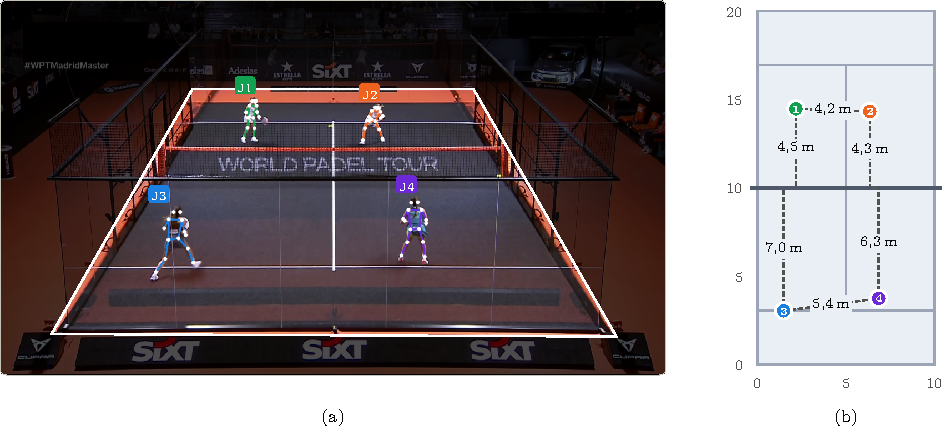
\includegraphics{figuras/jugadores}
  \caption{Fotograma de un punto (a). Resultado de la homografía con las distancias (b).}
  \label{fig:jugadores}
\end{figure}

Tras aplicar la máscara, en cada fotograma quedan solo los jugadores, pero falta saber cuál es cuál de un fotograma al siguiente.
El algoritmo de seguimiento ByteTrack~\cite{zhang2022bytetrack} hace justo esto, asignando un mismo identificador a la misma persona.
Predice dónde estará cada \textit{bounding box} y empareja por solapamiento.
Este algoritmo viene incluido en la biblioteca Ultralytics y se ejecuta en la misma llamada que el modelo de pose.
Cuando pierde a una persona, ByteTrack guarda su seguimiento durante un tiempo por si reaparece (en nuestra configuración, 120 fotogramas).
Si en ese tiempo no consigue volver a emparejarla, le asigna un identificador nuevo.

Para saber quién da cada golpe, cada jugador necesita que su identidad no cambie durante todo el punto: J1, J2, J3 y J4.
Estas se asignan durante los 3 primeros segundos del punto usando la posición media de los cuatro identificadores que aparecen en más fotogramas ~\cite{decorte2024padel}.
La numeración sigue el mismo criterio que las anotaciones del \textit{dataset}, lo que permite comparar con ellas el jugador que da cada golpe.

Cuando ByteTrack pierde a un jugador y le asigna un identificador nuevo, hay que decidir cuál de los cuatro es.
Como en la pista siempre hay cuatro jugadores, el identificador nuevo hereda la identidad del que falta.
Si falta más de un jugador, los nuevos heredan la de los jugadores ausentes cuya última posición conocida esté más cerca de donde aparecen.

\subsection{Pelota}
\label{sec:pelota}

El audio indica cuándo se produce cada golpe, pero no qué jugador lo da ni de qué tipo es.
Para resolver ambas preguntas es necesario conocer la posición de la pelota, ya que el golpe se asigna al jugador más cercano a ella, y además su trayectoria es una de las entradas del clasificador de golpes.
Para localizar la pelota en cada fotograma se utiliza una red propia basada en TrackNet~\cite{huang2019tracknet}, entrenada desde cero con partidos de pádel anotados~\cite{badanerin2026padeltracker100}.

La entrada de la red son tres fotogramas seguidos en los que se puede identificar a la pelota por su movimiento sobre un fondo estático.
La salida de la red es un mapa de calor donde cada celda indica, con un valor entre 0 y 1, la probabilidad de que la pelota se encuentre ahí.
La posición de la pelota es el centro de la celda de mayor valor que supere el umbral de 0,5; si ninguna lo supera, se considera que en ese fotograma no hay pelota (\cref{fig:mapa-calor}).
Cada celda del mapa equivale a un cuadrado de $10 \times 10$ píxeles del vídeo original, por lo que la posición tiene un margen de unos pocos píxeles.

\begin{figure}[htbp]
  \centering
  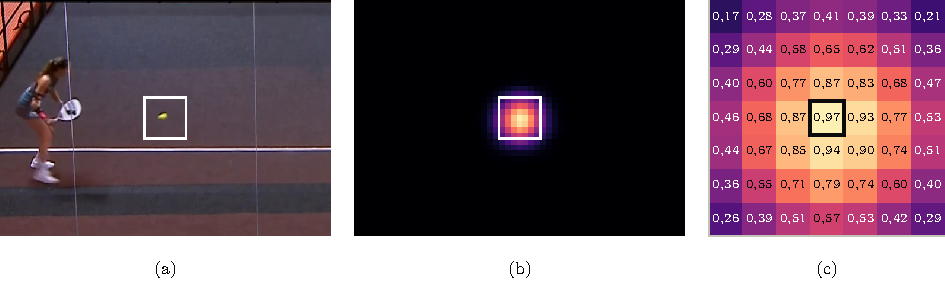
\includegraphics{figuras/mapa-calor}
  \caption{...}
  \label{fig:mapa-calor}
\end{figure}

La arquitectura base del modelo de detección de la pelota es una red adaptada del tipo U-Net~\cite{ronneberger2015unet}.
Dado que la U-Net se diseñó para segmentar imágenes biomédicas, una tarea que requiere precisión a nivel de píxel, se ha simplificado su estructura para localizar la pelota, como muestra la \cref{tab:red-pelota}.
En primer lugar, se ha reducido de cuatro a tres el número de veces que el codificador comprime la imagen.
En segundo lugar, se ha reducido de cuatro a uno el número de veces que el decodificador amplía la imagen.
Por último, se ha dividido el número de canales con el que empieza, de 64 a 32.
Estos cambios disminuyen el número de parámetros de unos 31 a 1,76 millones.
Además, se ha añadido un corrector en el paso final que ajusta el mapa de calor teniendo en cuenta también los fotogramas, pensado para situaciones donde la pelota esté tapada por un jugador.

\begin{table}[htbp]
  \centering
  \caption{...}
  \label{tab:red-pelota}
  \begin{tabular}{lcc}
\toprule
\textbf{} & \textbf{U-Net} & \textbf{Red propia} \\
\midrule
Número de veces que se reduce la imagen & 4 & 3 \\
Número de veces que se amplía la imagen & 4 & 1 \\
Canales (primer y último nivel) & $64 \to \num{1024}$ & $32 \to 256$ \\
Parámetros & 31\,M & 1,76\,M \\
\bottomrule
\end{tabular}

\end{table}

La red aprende comparando su salida ($p$) con un mapa objetivo ($t$), en el que todas las celdas valen cero salvo una mancha centrada en la pelota.
El error se mide con una entropía cruzada binaria ponderada, como media sobre las $N$ celdas del mapa:
\begin{equation}
  \mathcal{L} = -\frac{1}{N} \sum_{i=1}^{N} w_i \left[ t_i \log p_i + (1 - t_i) \log (1 - p_i) \right],
  \qquad w_i = 1 + 199\, t_i
\end{equation}
donde $w_i$ es el peso de cada celda: 1 en el fondo y hasta 200 en el centro de la pelota.
Sin estos pesos, como la pelota ocupa muy pocas celdas del mapa, la red podría aprender a devolver 0 en todas partes.

%En la práctica, la principal dificultad es que la pelota no siempre está a la vista: en los globos sale del encuadre, en ocasiones la tapa un jugador y en algunos fotogramas no llega a distinguirse aunque esté en juego.
%El sistema lo tolera porque ni la asignación ni el clasificador dependen de un único fotograma, como se explica en las siguientes secciones.

\subsection{Asignación del golpe}
\label{sec:asignacion}

Una vez localizada la pelota, el siguiente paso es asignar el golpe a un jugador.
Para ello se utilizan varios fotogramas alrededor del golpe~\cite{decorte2024padel}, de modo que la decisión no dependa de un único fotograma en el que pueda faltar la pelota o el jugador.
En cada uno se mide la distancia de la pelota a la muñeca de cada jugador, que recibe un voto con más peso cuanto más cerca está.
El golpe se atribuye al jugador que suma más votos.

Al analizar los fallos de este método se observó que se concentraban en los remates.
En un remate el jugador golpea la pelota por encima de la cabeza, lo que en la imagen la sitúa cerca de los jugadores del fondo.
Como estos aparecen más pequeños por la perspectiva, en píxeles parecen más cerca de ella de lo que realmente están.
Para corregirlo, la distancia se normaliza con la altura de la \textit{bounding box} de cada jugador, de modo que la medida sea comparable entre jugadores cercanos y lejanos.
La \cref{fig:asignacion} muestra cómo, sin esta corrección, el remate se atribuiría a J2 por la distancia en píxeles, mientras que con ella se atribuye a J4, que es quien golpea.
Con ella, el acierto en los remates pasa del 62~\% al 84~\%, lo que resuelve más de la mitad de sus fallos, y en el conjunto de los golpes, del 82,4~\% al 87,5~\%.

\begin{figure}[htbp]
  \centering
  % Generado por scripts/build_assignment_figure.py: no editar a mano.
\begin{minipage}[c]{0.52\linewidth}
  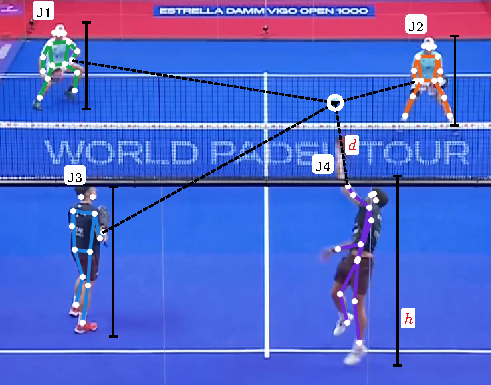
\includegraphics[width=\linewidth]{figuras/asignacion-fotograma}
\end{minipage}\hfill
\begin{minipage}[c]{0.45\linewidth}
  \centering
  \begin{tabular}{lccc}
  \toprule
  \textbf{} & \textbf{$d$ (px)} & \textbf{$h$ (px)} & \textbf{$d/h$} \\
  \midrule
  J1 & 402 & 130 & 3,09 \\
  J2 & \textbf{124} & 135 & 0,92 \\
  J3 & 400 & 225 & 1,78 \\
  J4 & 128 & 286 & \textbf{0,45} \\
  \bottomrule
  \end{tabular}
\end{minipage}

  \caption{...}
  \label{fig:asignacion}
\end{figure}

La ventana se fijó en 9 fotogramas, 4 antes y 4 después del golpe.
Ampliarla empeora el acierto (87,5~\% con $\pm 4$, 86,8~\% con $\pm 5$ y 85,6~\% con $\pm 6$), porque los fotogramas alejados del golpe dan el voto a quien está cerca de la pelota en ese momento, no por quien golpeó.

\subsection{Tipo de golpe}
\label{sec:tipo}

El último paso del flujo utiliza todo lo obtenido anteriormente para clasificar cada golpe.
Esto convierte la detección en información útil para analizar el juego, como cuántos golpes de cada tipo da cada jugador y desde dónde los ejecuta.
Es, además, la base de análisis más completos: conociendo el tipo de cada golpe se podría estudiar, por ejemplo, en qué golpe se pierden más puntos o qué patrones se repiten antes de un error, y llegar a que un sistema saque conclusiones de un partido por sí mismo.
Cada golpe se clasifica en uno de cuatro tipos: saque, derecha, revés o remate. Se eligieron estas clases por ser las familias básicas de golpes del pádel, y son el punto de partida necesario: una vez se distinguen de forma fiable, cada una puede subdividirse después, por ejemplo, separando dentro de los remates la bandeja y la víbora, sin rehacer el resto del sistema.
El clasificador parte de BST~\cite{chang2026bst}, un modelo propuesto para el bádminton.
Llevarlo al pádel, con cuatro jugadores en pista y otros tipos de golpe, ha exigido adaptar qué recibe el modelo, qué clases distingue y con qué datos se entrena.

Un golpe se reconoce por el movimiento completo del jugador y no por un único fotograma, por lo que el clasificador analiza un intervalo de vídeo alrededor de cada golpe.
La forma más directa de definir ese intervalo es una ventana de duración fija centrada en el golpe, pero el tiempo entre golpes consecutivos varía a lo largo del punto.
Una ventana corta puede no abarcar el gesto completo, mientras que una ventana larga incorpora otros golpes alejados del que se pretende clasificar.

Para resolver este problema se adopta una ventana adaptativa, cuyos límites se definen a partir de los golpes vecinos (\cref{fig:ventana}).
De este modo, la ventana contiene tanto la preparación del jugador como la ejecución del golpe.
Adicionalmente, y para que un intervalo largo entre golpes no introduzca un exceso de información que pudiera dificultar la clasificación correcta, ningún extremo se aleja más de 1,5~s del golpe.
En el primer y el último golpe del punto, que carecen de golpe anterior o siguiente, el extremo correspondiente se sitúa a 0,5~s del golpe.
Por último, como la duración de la ventana varía de un golpe a otro, se toman siempre 100 fotogramas repartidos uniformemente a lo largo de ella, repitiendo o descartando fotogramas si procede, de forma que todas las ventanas tengan la misma longitud.

\begin{figure}[htbp]
  \centering
  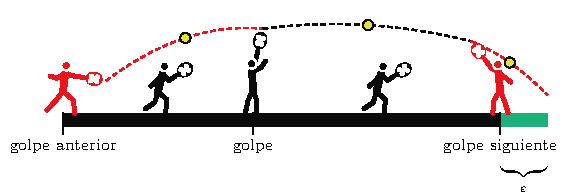
\includegraphics{figuras/ventana}
  \caption{...}
  \label{fig:ventana}
\end{figure}

De cada ventana se extraen dos secuencias, la pose del jugador que golpea y la posición de la pelota (\cref{fig:entrada}).
En cada fotograma, la pose se expresa respecto al punto medio de las caderas, de modo que no depende de la posición del jugador en la imagen.
Como ya se comentó en la asignación (\cref{sec:asignacion}), para corregir el efecto de la perspectiva es necesario normalizar la posición relativa de cada punto del esqueleto.
Esto se logra dividiendo las coordenadas de cada uno de los 17 puntos por la longitud del tronco.
Así, todos los esqueletos quedan a la misma escala, y un mismo gesto produce los mismos valores en un jugador cercano y en uno lejano.
La pelota se normaliza con la misma referencia, tomando la posición y la escala medias del jugador en la ventana.
Así, el modelo no recibe la posición de la pelota en píxeles, sino su posición relativa al jugador.

\begin{figure}[htbp]
  \centering
  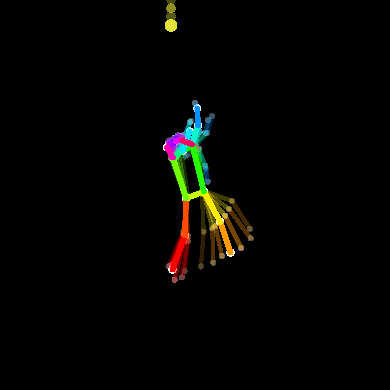
\includegraphics{figuras/entrada}
  \caption{...}
  \label{fig:entrada}
\end{figure}

Cuando la pelota no se detecta en un fotograma, sus coordenadas valen cero y un indicador adicional señala su ausencia, ya que, de otro modo, el modelo interpretaría ese cero como una posición real.
Si el detector pierde al jugador en algún paso de la ventana, se mantiene su último esqueleto conocido, puesto que una pose a cero también se interpretaría como una pose real.
Si el jugador aparece en menos de la cuarta parte de los pasos, la ventana no contiene información suficiente y el golpe se queda sin clasificar.
Por último, las ventanas de entrenamiento se construyen a partir de las mismas salidas que el sistema produce en funcionamiento. Del etiquetado proceden únicamente el tipo de golpe y su instante.
De este modo, el modelo aprende con los mismos errores que encontrará después, y no con poses perfectas que el sistema nunca le proporcionará.

A continuación se describe cada módulo de la red en detalle. La \cref{fig:clasificador} muestra el flujo que recorren los datos.

\begin{figure}[htbp]
  \centering
  % Arquitectura del clasificador de tipo de golpe (sección «Tipo de golpe»), al
% estilo del recuadro BST-0 de la figura 2 de BST, con los colores de la memoria
% y los iconos del jugador y la pelota en lugar de cajas para las entradas (con
% sus dimensiones, sin nombre: el icono ya dice qué es). Las dimensiones van con
% la notación del texto y de las ecuaciones: T pasos, J puntos clave, D dimensión
% del modelo y C clases.
% Sigue a ShotTypeBST (padel_ml.shot_type_model): un TCN por secuencia, un
% codificador temporal con los mismos pesos para las dos, la atención cruzada
% (Q de la pose; K y V de la pelota), el codificador de interacción y la cabeza
% sobre los tres resúmenes. Colores, estilos e iconos en config/config.tex.
\begin{adjustbox}{max width=\linewidth}
\begin{tikzpicture}[
  op/.style={circle, draw=tinta2, fill=white, line width=0.5pt, minimum size=3.6mm,
    inner sep=0pt, font=\scriptsize, text=tinta},
  token/.style={draw=tinta2, fill=white, line width=0.5pt, minimum size=2.4mm, inner sep=0pt},
  rama/.style={circle, fill=tinta2, minimum size=1.3mm, inner sep=0pt},
  alta/.style={caja, minimum height=31mm},
  modulo/.style={caja, text width=10mm},
  nombre/.style={font=\footnotesize, text=tinta, inner sep=1pt, align=center},
  pics/posicion/.style={code={
    \node[op] (-c) {};
    \draw[tinta2, line width=0.45pt]
      plot[domain=-0.12:0.12, samples=25, smooth] (\x, {0.065*sin(\x/0.12*180)});
  }},
]
  \def\yP{1.15}
  \def\yB{-1.15}
  \def\yR{2.15}

  % Entradas: el jugador que golpea y la pelota
  \pic[scale=1.25] at (0,\yP-0.12) {jugador=tinta};
  \node[nombre, below, font=\scriptsize, text=tenue] at (0,\yP-0.16) {$T\times J\times3$};
  \pic[scale=1.7] at (0,\yB+0.2) {pelota=pelota};
  \node[nombre, below, font=\scriptsize, text=tenue] at (0,\yB-0.04) {$T\times3$};
  \node[modulo] (tcnP) at (1.75,\yP) {TCN};
  \node[modulo] (tcnB) at (1.75,\yB) {TCN};
  \draw[flecha] (0.55,\yP) -- (tcnP);
  \draw[flecha] (0.55,\yB) -- (tcnB);

  % Token de clase y codificación posicional antes del codificador temporal
  \foreach \r/\y in {P/\yP, B/\yB} {
    \node[op] (cat\r) at (2.85,\y) {$\|$};
    \node[token] (tok\r) at (2.85,\y+0.5) {};
    \node[op] (sum\r) at (3.4,\y) {$+$};
    \pic (pe\r) at (3.4,\y-0.5) {posicion};
    \draw[flecha] (tcn\r) -- (cat\r);
    \draw[flecha] (tok\r) -- (cat\r);
    \draw[flecha] (cat\r) -- (sum\r);
    \draw[flecha] (pe\r-c) -- (sum\r);
  }

  \node[alta, text width=17mm] (enc1) at (4.75,0)
    {Codificador\\temporal\subcaja{2 capas}\subcaja{mismos pesos}};
  \draw[flecha] (sumP) -- (sumP -| enc1.west);
  \draw[flecha] (sumB) -- (sumB -| enc1.west);

  % Se separa el resumen (token) de la secuencia, que sigue
  \node[rama] (sP) at (6.0,\yP) {};
  \node[rama] (sB) at (6.0,\yB) {};
  \draw[linea] (enc1.east |- sP) -- (sP);
  \draw[linea] (enc1.east |- sB) -- (sB);

  \node[alta, text width=15mm] (cross) at (8.6,0) {Atención\\cruzada\subcaja{1 capa}};
  \node[op] (sum2P) at (7.15,\yP) {$+$};
  \pic (pe2P) at (7.15,\yP-0.5) {posicion};
  \node[op] (sum2B) at (7.15,\yB) {$+$};
  \pic (pe2B) at (7.15,\yB-0.5) {posicion};
  \draw[flecha] (sP) -- (sum2P) node[pos=0.5, above, font=\scriptsize, text=tenue] {$T\times D$};
  \draw[flecha] (sB) -- (sum2B) node[pos=0.5, above, font=\scriptsize, text=tenue] {$T\times D$};
  \draw[flecha] (pe2P-c) -- (sum2P);
  \draw[flecha] (pe2B-c) -- (sum2B);
  \draw[flecha] (sum2P) -- (sum2P -| cross.west) node[pos=0.5, above, font=\scriptsize] {$Q$};
  \draw[flecha] (sum2B) -- (sum2B -| cross.west) node[pos=0.5, above, font=\scriptsize] {$K, V$};

  % Codificador de interacción sobre la secuencia fusionada
  \node[op] (catF) at (10.0,0) {$\|$};
  \node[token] (tokF) at (10.0,0.5) {};
  \node[op] (sumF) at (10.55,0) {$+$};
  \pic (peF) at (10.55,-0.5) {posicion};
  \node[caja, text width=21mm] (enc2) at (12.15,0) {Codificador\\de interacción\subcaja{1 capa}};
  \draw[flecha] (cross) -- (catF);
  \draw[flecha] (tokF) -- (catF);
  \draw[flecha] (catF) -- (sumF);
  \draw[flecha] (peF-c) -- (sumF);
  \draw[flecha] (sumF) -- (enc2);

  % Cabeza: los tres resúmenes, concatenados
  \node[op] (head) at (13.75,0) {$\|$};
  \node[modulo] (mlp) at (14.75,0) {MLP};
  \node[entrada, text width=12mm] (out) at (16.2,0) {$C$ valores\subcaja{uno por clase}};
  \draw[flecha] (sP) -- (6.0,\yR) -| (head);
  \draw[flecha] (sB) -- (6.0,-\yR) -| (head);
  \pic[scale=0.8] at (9.6,\yR+0.08) {jugador=tinta};
  \node[dato, anchor=west] (rP) at (9.8,\yR+0.18) {resumen de la pose};
  \pic[scale=1.1] at (9.6,-\yR-0.2) {pelota=pelota};
  \node[dato, anchor=west] (rB) at (9.8,-\yR-0.2) {resumen de la pelota};
  \draw[flecha] (enc2) -- (head);
  \draw[flecha] (head) -- (mlp);
  \draw[flecha] (mlp) -- (out);

  \begin{scope}[on background layer]
    \node[panel, fill=panelgolpe, fit={(-0.75,0) (out) (rP) (rB) (6.0,2.75) (6.0,-2.6)}] (g) {};
  \end{scope}

  % Leyenda, centrada bajo el panel
  \begin{scope}[shift={($(g.south)+(-7.75,-0.45)$)},
      leyenda/.style={font=\scriptsize, text=tinta2, anchor=west, inner sep=1pt}]
    \node[token] (l1) at (0,0) {};
    \node[leyenda, right=1mm of l1] (t1) {token de clase};
    \node[op, right=5mm of t1] (l2) {$\|$};
    \node[leyenda, right=1mm of l2] (t2) {concatenación};
    \node[op, right=5mm of t2] (l3) {$+$};
    \node[leyenda, right=1mm of l3] (t3) {suma};
    \path (t3.east) ++(6.8mm,0) pic (l4) {posicion};
    \node[leyenda, right=1mm of l4-c] (t4) {codificación posicional};
    \node[rama, right=5mm of t4] (l5) {};
    \node[leyenda, right=1mm of l5] {se separa el resumen de la secuencia};
    \node[leyenda] at (-0.12,-0.45)
      {$T$: pasos \quad $J$: puntos clave \quad $D$: dimensión del modelo \quad $C$: clases};
  \end{scope}
\end{tikzpicture}
\end{adjustbox}

  \caption{...}
  \label{fig:clasificador}
\end{figure}

El primer módulo de la red es una \textbf{\ac{tcn}}~\cite{bai2018tcn}, que se encarga de convertir posiciones en movimiento.
La \ac{tcn} calcula cada paso a partir de él y de sus vecinos.
Con esto, cada paso puede recoger hacia dónde se mueven los puntos del cuerpo y la pelota, algo que una posición aislada no contiene.
Además, lleva las dos secuencias, de 51 y 3 valores por paso, a un mismo tamaño $D$, ya que los módulos siguientes las comparan entre sí y las procesan con los mismos pesos.
Para cada filtro de tamaño $k$, la salida en el paso $s$ es:
\begin{equation}
  F(s) = \sum_{i=0}^{k-1} f(i)\, x_{s + d\,(i - \lfloor k/2 \rfloor)},
  \label{eq:tcn}
\end{equation}
donde $f(i)$ son los $k$ pesos del filtro, aprendidos durante el entrenamiento, y $d$ es la dilatación, la separación entre las posiciones que mira.
Cada filtro aplica esta operación a todos los valores de entrada y suma los resultados, y hay $D$ filtros, uno por cada valor de salida.
La dilatación es lo que permite cubrir más pasos sin más pesos o capas.
La \ac{tcn} tiene dos capas: en la primera la salida resume 5 pasos seguidos; en la segunda mira 5 de esas salidas separadas de 3 en 3.
Así, cada paso abarca 17 pasos de la entrada, frente a los 9 que cubrirían dos capas sin dilatación.

El \textbf{token de clase} es un vector que se añade al principio de la secuencia y que la red aprende durante el entrenamiento, como el resto de sus pesos.
Su función es resumir la secuencia entera, ya que la cabeza necesita un único vector para decidir y tras la \ac{tcn} hay 100.

La \textbf{codificación posicional} es un vector que se encarga de comunicar al codificador en qué orden van los pasos, sumando a cada paso una firma de su posición.
Es necesaria porque, sin ella, el codificador no distinguiría el orden de los pasos, y para clasificar un golpe importa el orden de la preparación, el impacto y el cierre.
Se utiliza la codificación sinusoidal del Transformer~\cite{vaswani2017attention}, que, para el paso en la posición $t$ y cada pareja de dimensiones $i$, de 0 a $D/2-1$, es:
\begin{equation}
  \mathrm{PE}(t, 2i) = \sin\!\left(\frac{t}{10000^{2i/D}}\right), \qquad
  \mathrm{PE}(t, 2i+1) = \cos\!\left(\frac{t}{10000^{2i/D}}\right).
  \label{eq:posicional}
\end{equation}
Cada pareja de dimensiones oscila a una frecuencia distinta: las primeras cambian muy rápido de un paso al siguiente y las últimas muy despacio, y la combinación de todas da una firma única para cada posición.
Las posiciones cercanas tienen firmas parecidas, así que la red puede tener en cuenta la distancia entre pasos.
Esta codificación se suma antes de cada uno de los tres módulos que siguen en la figura.

El \textbf{codificador temporal} es una pila de dos capas de transformer, cada una formada por una atención y una \ac{ffn}.
Se encarga de relacionar cada paso con todos los demás de la ventana, no solo con sus vecinos.
El codificador permite, por ejemplo, que el paso del impacto tome información de la preparación de un segundo antes.
Además, no todos los pasos aportan lo mismo: el codificador aprende cuánta información toma cada paso de cada uno de los demás, de modo que un paso en el que el jugador espera pesa menos que el impacto.

Cada paso de la secuencia $X$ produce tres vectores, multiplicándose por tres matrices aprendidas:
\begin{itemize}
  \item $Q$ (consulta): lo que el paso busca.
  \item $K$ (clave): con lo que se le puede encontrar.
  \item $V$ (valor): el contenido que aporta si se le elige.
\end{itemize}
\begin{equation}
  Q = XW_Q, \qquad K = XW_K, \qquad V = XW_V,
  \qquad
  \text{Atención}(Q, K, V) = \mathrm{softmax}\!\left(\frac{QK^\top}{\sqrt{D_A}}\right) V,
  \label{eq:atencion}
\end{equation}
Es decir, se compara lo que busca cada paso con lo que ofrecen los demás, y cada paso recibe una media de sus contenidos ponderada por ese parecido.

La atención de cada capa se repite 6 veces en paralelo, cada una con sus propias matrices, y cada repetición se denomina cabeza.
Con una sola cabeza, cada paso repartiría su atención de una única manera, pero en un golpe hay varias relaciones a la vez: el impacto se relaciona con la preparación y también con la llegada de la pelota.
Con varias, cada cabeza puede especializarse en una relación distinta.
Las salidas de todas se concatenan y se combinan en un único vector por paso, la atención multicabeza (\ac{mhsa}):
\begin{equation}
  \mathrm{MHSA}(X) = \big[\,\mathrm{cabeza}_1 \,\|\, \cdots \,\|\, \mathrm{cabeza}_H\,\big]\, W_O,
  \label{eq:multicabeza}
\end{equation}
donde $H$ es el número de cabezas y $W_O$, la matriz que las combina.

La segunda parte de cada capa, la \ac{ffn}, es una red pequeña que procesa cada paso por separado: la atención reúne información de los demás pasos y la \ac{ffn} la transforma.
Antes de cada parte se normalizan los valores y a su salida se suma lo que había a la entrada, lo que facilita el entrenamiento al apilar capas.
El mismo codificador, con los mismos pesos, procesa por separado la pose y la pelota.
Como el token también participa en la atención y no tiene contenido propio, a la salida contiene el resumen de la secuencia, que va directamente a la cabeza, mientras que los demás pasos continúan hacia la atención cruzada.



\section{Visor web}
\label{sec:visor}


\chapter{Experimentos y validación}
\label{cap:experimentos}
% !TEX root = ../tfg.tex

\alumno{Extensión prevista: unas 12 páginas. Todas las cifras y figuras salen de docs/metrics/; ninguna se escribe a mano.}

\section{Protocolo y métricas}

\section{Resultados de cada paso por separado}
\alumno{Y la comparación con el trabajo de referencia, solo donde la prueba es la misma.}

\section{El sistema completo}
\alumno{Evaluado dejando cada torneo fuera del entrenamiento.}

\section{Análisis de errores}
\alumno{Confusiones entre tipos, el cruce de identidades de VIGO\_00, resultados por torneo.}

\section{Decisiones medidas}
\alumno{La ventana de voto, la resolución de la pelota, los pesos de clase y la regla del saque.}

\section{Coste computacional}

\section{Limitaciones}
\alumno{Fuente: docs/sistema.md, sección de limitaciones.}


\chapter{Conclusiones y trabajo futuro}
\label{cap:conclusiones}
% !TEX root = ../tfg.tex

\alumno{Extensión prevista: unas 3 páginas.}

\section{Objetivos y resultados}
\alumno{Cada objetivo específico frente a lo conseguido.}

\section{Lecciones aprendidas}

\section{Trabajo futuro}


%%%%%%%%%%%%%%%%%%%%%%%%%%%%%%% Bibliografía %%%%%%%%%%%%%%%%%%%%%%%%%%%%%%%

\cleardoublepage
\phantomsection
\addcontentsline{toc}{chapter}{Bibliografía}

\footnotesize{
\bibliographystyle{IEEEtran}
\bibliography{bibliografia}
}

\normalsize
\raggedbottom

%%%%%%%%%%%%%%%%%%%%%%%%%%%%%%% Anexos %%%%%%%%%%%%%%%%%%%%%%%%%%%%%%%

\cleardoublepage
\appendix

\phantomsection
\addcontentsline{toc}{chapter}{Anexos}

\mbox{}
\vfill
\begin{center}
\begin{Huge}
\textbf{Anexos}
\end{Huge}
\end{center}
\vfill
\mbox{}
\thispagestyle{empty}

\newpage
\mbox{}
\thispagestyle{empty}
\newpage

\chapter{Reproducibilidad}
\label{anexo:reproducibilidad}
% !TEX root = ../../tfg.tex

\alumno{Estructura del repositorio, cómo instalarlo y cómo regenerar cada cifra. Fuente: README.md y docs/metrics/README.md.}


\chapter{Registro de decisiones}
\label{anexo:decisiones}
% !TEX root = ../../tfg.tex

\alumno{Índice de las decisiones de arquitectura (ADR) con su estado. Fuente: docs/decisions/README.md.}


\chapter{Herramientas de etiquetado}
\label{anexo:etiquetado}
% !TEX root = ../../tfg.tex

\alumno{Las herramientas propias de etiquetado del tipo de golpe y de marcado de la pista, con capturas (docs/media/).}


\chapter{Visor web}
\label{anexo:visor-web}
% !TEX root = ../../tfg.tex

\alumno{Capturas del visor web (docs/media/).}


\chapter{Uso de herramientas de inteligencia artificial}
\label{anexo:uso-ia}
% !TEX root = ../../tfg.tex

\alumno{Pendiente de la respuesta del tutor sobre si incluir esta sección y dónde.}


\end{document}
